\documentclass[aspectratio=169]{beamer}
\usetheme{Singapore}

\usepackage{cmap}
\usepackage[french]{babel}
\usepackage[T1]{fontenc}
\usepackage[utf8]{inputenc}
\usepackage[kerning=true]{microtype}
\usepackage{lmodern}

\usepackage{amsmath}
\usepackage{amsfonts}
\usepackage{amssymb}
\usepackage{amsthm}

\usepackage{mathtools}
\usepackage{wrapfig}
\usepackage{enumitem}

\uselanguage{French}
\languagepath{French}

%\usepackage{graphicx}

%\graphicspath{{./../report/images/}}

\AtBeginSection[]
{
  \begin{frame}
    \frametitle{Plan}
    \tableofcontents[currentsection]
  \end{frame}
}

\theoremstyle{plain}
%\newtheorem*{theorem}{Theorem}
%\newtheorem*{example}{Example}
\newtheorem*{remark}{Remarque}
\theoremstyle{definition}
%\newtheorem*{definition}{Definition}
\newtheorem*{thesis}{Thèse}

\DeclarePairedDelimiter\ket{\lvert}{\rangle}

\title{\textbf{Calcul et informatique quantique:\\une introduction formelle}}
\author{Antoine Groudiev}
\institute{ENS Ulm}
\date{18 Janvier 2024}

\begin{document}
\frame{\titlepage}

\begin{frame}{Plan}
    \tableofcontents
\end{frame}

\section{Modèles de calcul quantiques}

\subsection{Introduction à l'informatique quantique}
\begin{frame}{Introduction}
    On manipule non pas des \emph{bits}, mais des \emph{qubits}.
    \begin{definition}[Superposition quantique]        
        \begin{equation*}
            \ket{\Psi}=\alpha\ket{\Psi}+\beta\ket{\Psi}
        \end{equation*}
        où $\alpha, \beta\in \mathbb{C}$ sont appelés les \emph{amplitudes d'états}. 
    \end{definition}

    \begin{remark}[Condition de normalisation]
        \begin{equation*}
        |\alpha|^2+|\beta|^2=1
        \end{equation*}
    \end{remark}
\end{frame}

\subsection{Circuits quantiques}
\begin{frame}{Circuits quantiques}
    \begin{figure}[!ht]
        \centering
        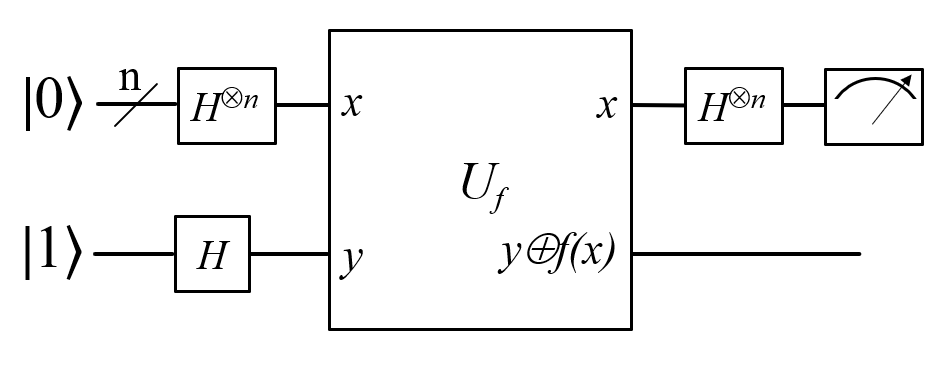
\includegraphics[scale=0.5]{deutsch-circuit-n.png}
        \caption{Un exemple de circuit (Algorithme de Deutsch-Jozsa)}
    \end{figure}
\end{frame}

\begin{frame}{Porte $X$}
    \begin{equation*}
        X : \alpha\ket{0} + \beta\ket{1} \mapsto \beta\ket{0} + \alpha\ket{1}
    \end{equation*}
    Sous forme de matrice:
    \begin{equation*}
        X \cong \begin{pmatrix}
            0&1\\
            1&0
        \end{pmatrix}
    \end{equation*}
\end{frame}

%\begin{frame}{Porte $Z$}
%    \begin{equation*}
%        Z : \alpha\ket{0} + \beta\ket{1} \mapsto \alpha\ket{0} - \beta\ket{1}
%    \end{equation*}
%    Sous forme de matrice:
%    \begin{equation*}
%        Z \cong \begin{pmatrix}
%            1&0\\
%            0&-1
%        \end{pmatrix}
%    \end{equation*}
%\end{frame}

\begin{frame}{Porte de Hadamard}
    \begin{equation*}
        H \cong \frac{1}{\sqrt{2}}
        \begin{pmatrix}
            1&1\\
            1&-1
        \end{pmatrix}
    \end{equation*}
    Résultat direct:
    \begin{equation*}
        \begin{cases}
            H\ket{0} = \frac{1}{\sqrt{2}}(\ket{0}+\ket{1}) \\
            H\ket{1} = \frac{1}{\sqrt{2}}(\ket{0}-\ket{1})
        \end{cases}
    \end{equation*}
    \begin{figure}
        \label{fig:basic-circuit}
        \centering
        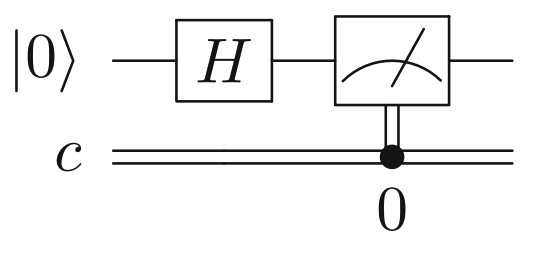
\includegraphics[scale=0.3]{basic-circuit.png}
    \end{figure}
\end{frame}

%\begin{frame}{Intrication quantique}
%\end{frame}
%
%\begin{frame}{Porte $CNOT$}
%\end{frame}

\subsection{Langages, automates, grammaires quantiques}
\begin{frame}{Langage quantique}
    \framesubtitle{Retour sur les langages classiques}
    Soit $\Sigma$ un alphabet, et $L\subseteq \Sigma^\star$ un langage. $L$ peut être défini alternativement comme un sous-ensemble de $\Sigma^\star$, ou par sa fonction caractéristique $\chi_L$:
    \begin{equation*}
        \chi_L(w) = \begin{cases*}
            1 & si $w\in L$\\
            0 & sinon
        \end{cases*}
    \end{equation*}
\end{frame}

\begin{frame}{Langage quantique}
    \framesubtitle{Définition}
    On peut par analogie définir un \emph{langage quantique} comme une fonction associant des probabilités à des mots:
    \begin{definition}[Langage quantique]
        Un \emph{langage quantique} sur l'alphabet $\Sigma$ est une fonction $f$ telle que:
        \begin{equation*}
            f : \Sigma^\star \to [0, 1]
        \end{equation*}
        
    \end{definition}

    \begin{remark}
        $f$ est un langage classique lorsque $f(\Sigma^\star) \subseteq \{0, 1\}$.
    \end{remark}
\end{frame}

\begin{frame}{Automate quantique fini}
    \begin{definition}[AQF]
        Un \emph{Automate Quantique Fini} $\mathcal{A}=(H, s_{\textnormal{init}}, H_{\textnormal{accept}}, P_{\textnormal{accept}}, \Sigma, \delta)$ consiste en:
        \begin{enumerate}[label=--, noitemsep]
            \item un espace de Hilbert $H$ de dimension $n$
            \item un vecteur initial normalisé $s_{\textnormal{init}}\in H$ (i.e. $\|s_{\textnormal{init}}\|^2=1$)
            \item un sous-espace $H_{\textnormal{accept}} \subseteq H$, et un opérateur $P_{\textnormal{accept}}$ projettant sur $H_{\textnormal{accept}}$
            \item un alphabet $\Sigma$
            \item une fonction $\delta : \Sigma \to U_n(\mathbb{C})$, associant à chaque lettre une matrice unitaire $U_a$ (c'est-à-dire $U_aU_a^\dagger = I_n$)
        \end{enumerate}
        
        On note $\delta^\star(w=w_1\cdots w_{|w|}) = \delta(w_{|w|})\cdots \delta(w_1) = U_{w_{|w|}}\cdots U_{w_1}$. Enfin, le langage reconnu par $\mathcal{A}$ est:
        \begin{equation*}
            f_{\mathcal{A}} : w \mapsto \|P_{\textnormal{accept}}\delta^\star(w)s_{\textnormal{init}}\|^2
        \end{equation*}
    \end{definition}
\end{frame}

%\begin{frame}{Langage quantique régulier et propriétés}
%    \begin{definition}[LQR]
%        Un \emph{Langage Quantique Régulier} est un langage quantique reconnu par un automate quantique fini
%    \end{definition}
%
%    \begin{theorem}[Clôture des LQR par produit]
%        Soient $f, g$ des LQRs. Alors, le produit $fg$ est un LQR.
%    \end{theorem}
%
%    \begin{theorem}[Clôture des LQR par combinaison linéaire]
%        Soient $f_i$ des LQRs, et $c_i$ des constantes telles que $\sum_i c_i \leq 1$. Alors, $\sum_i c_if_i$ est un LQR.
%    \end{theorem}
%\end{frame}
%
%\begin{frame}{Langage quantique régulier et propriétés}
%    \begin{theorem}[Lemme de pompage quantique]
%        Si $f$ est un LQR, alors pour tout mot $w\in\Sigma^\star$ et tout $\varepsilon > 0$, il existe $k\in \mathbb{N}^\star$ tel que $\|f(uw^kv) - f(uv)\| < \varepsilon$ pour tout mots $u, v$. De plus, si l'automate de $f$ est de dimension $n$, alors il existe une constante $c$ (indépendante de $\varepsilon$) telle que $k < (c\varepsilon)^{-n}$.
%    \end{theorem}
%\end{frame}
%
%\begin{frame}{Grammaire quantique hors-contexte}
%    \begin{definition}[Grammaire\footnote{\url{https://xkcd.com/1090/}} Quantique Hors-Contexte]
%        Une \emph{Grammaire Quantique Hors-Contexte} $G=(V, T, I, P)$ de \emph{dimensionnalité} $n$ consiste en:
%        \begin{itemize}[label=--, noitemsep]
%            \item un alphabet $V$ de variables
%            \item un alphabet $T$ de terminaux
%            \item une variable initiale $I\in V$
%            \item un ensemble fini de productions $P$ de la forme $\alpha\to \beta$, où $(\alpha, \beta)\in V\times (T\cup V)^\star$.
%        \end{itemize}
%        
%    \end{definition}
%\end{frame}
%
%\begin{frame}
%    À chaque production de $P$ est associée un ensemble d'amplitudes complexes $\left(c_k(\alpha\to\beta)\right)_{1\leq k\leq n}$.
%    
%    On définit l'amplitude d'\emph{une} suite de productions:
%    \begin{equation*}
%        c_k(\alpha_1 \to \dots \to \alpha_m=\beta) := \prod_{i=1}^{m-1} c_k(\alpha_i\to\alpha_{i+1})
%    \end{equation*}
%
%    Et l'amplitude d'une dérivation:
%    \begin{equation*}
%        c_k(\alpha\Rightarrow\beta) := \sum_{\alpha=\alpha_1 \to \dots \to \alpha_m=\beta} c_k(\alpha_1 \to \dots \to \alpha_m)
%    \end{equation*}
%
%    Enfin, $G$ \emph{génère} le langage quantique $f$ définit par:
%    \begin{equation*}
%        f(w) = \sum_{k=1}^n \|c_k(I\Rightarrow w)\|^2
%    \end{equation*}
%\end{frame}
%
%\begin{frame}{Automate à pile quantique}
%    \begin{definition}[QPDA]
%        Un \emph{Automate à Pile Quantique} $\mathcal{A}=(H=Q\otimes \Sigma, \Gamma, Q_{\textnormal{acccept}}, s_{\textnormal{init}}, A, \delta)$ consiste en:
%        \begin{itemize}[label=--, noitemsep]
%            \item un espace de Hilbertt $H$ des configurations de $\mathcal{A}$, avec $H=Q\otimes \Sigma$ pour $Q$, $\Sigma$
%            \item chaque vecteur de base de $\Sigma$ est un mot fini de \emph{l'alphabet de pile} $\Gamma$
%            \item un état initial $s_{\textnormal{init}}$
%            \item $Q_{\textnormal{acccept}} \subseteq Q$, tel que $H_{\textnormal{acccept}}=Q_{\textnormal{acccept}}\otimes \{\varepsilon\}$
%            \item un alphabet d'entrée $A$
%            \item une fonction de transition $\delta$, telle que $\forall a\in A$, $\delta(a)$ est un endomorphisme unitaire
%        \end{itemize}
%    \end{definition}
%\end{frame}
%
%\begin{frame}{Automate à pile quantique}
%    \framesubtitle{(Suite)}
%    Pour s'assurer du comportement LIFO de la pile, on ajoute les contraintes suivantes:
%    Soient $q_1, q_2\in Q$ des états de contrôle, et $\sigma_1, \sigma_2\in \Gamma$ des états de la pile; l'amplitude de la transition $(q_1, \sigma_1)$ to $(q_2, \sigma_2)$ est non-nulle seulement s'il existe $t\in T$ tel que:
%    \begin{equation*}
%        (\sigma_1t = \sigma_2) \lor (\sigma_1 = \sigma_2t) \lor (\sigma_1 = \sigma_2)
%    \end{equation*}
%    De plus, les amplitudes de transition peuvent dépendre uniquement de la dernière lettre de $\sigma_1$ et de $\sigma_2$.
%
%    Le langage reconnu par $\mathcal{A}$ est la fonction:
%    \begin{equation*}
%        f_{\mathcal{A}} : w \mapsto \|P_{\textnormal{accept}}\delta^\star(w)s_{\textnormal{init}}\|^2
%    \end{equation*}
%\end{frame}
%
%\begin{frame}{Théorème d'équivalence}
%    \begin{theorem}[Équivalence entre GQHC et APQ]
%        Un langage quantique est généré par une grammaire quantique hors-contexte si et seulement si il est reconnu par un automate à pile quantique.
%    \end{theorem}
%\end{frame}

\begin{frame}{Machine de Turing quantique}
    \begin{definition}[MTQ] Une \emph{Machine de Turing Quantique} $M = (H, \Gamma, b, \Sigma, \delta, q_0, Q_{\textnormal{accept}})$ consiste en:
        \begin{enumerate}[label=--, noitemsep]
            \item un espace de Hilbert $Q$ des états
            \item un autre espace de Hilbert $\Gamma$ de la bande
            \item un symbole blanc $\sqcup\in \Gamma$
            \item un alphabet d'entrée et de sortie $\Sigma$
            \item un état (vecteur) initial $q_0\in Q$
            \item un sous-espace $Q_{\textnormal{accept}}\subseteq Q$
            \item une fonction de transition $\delta$ telle que:
            \begin{equation*}
                \delta : \Sigma \times Q\otimes \Gamma \to \Sigma \times Q\otimes \Gamma \times \{L, R\}
            \end{equation*}
        \end{enumerate}
    \end{definition}
\end{frame}

\section{Théorie de la complexité quantique}
\subsection{Classe BQP}
\begin{frame}{Classe BQP (Bounded-error Quantum Polynomial time)}
    \begin{definition}[BQP] 
        La classe \emph{Bounded-error Quantum Polynomial time} (BQP) est l'ensemble des problèmes de décision qui peuvent être résolus en temps polynomial par une machine de Turing quantique, avec une erreur maximale de $\frac{1}{3}$. 
    \end{definition}
\end{frame}

%\begin{frame}{Un problème Promise-BQP-complet}
%    \begin{definition}[Problème APPROX-QCIRCUIT-PROB]
%        \textsc{Entrée}: $\alpha, \beta$ tels que $0\leq\beta<\alpha\leq 1$, et la description d'un circuit quantique $C$ tel que:
%        \begin{itemize}[label=--, noitemsep]
%            \item le circuit prend en entrée $n$ qubits
%            \item le circuit contient $m$ portes
%            \item $m$ est polynomial en $n$
%            \item la probabilité $P$ de mesurer le premier qubit du circuit initialisé à $\ket{0}^{\otimes n}$, est telle que $P\geq\alpha$ ou $P\leq\beta$
%        \end{itemize}
%        \textsc{Sortie}: Déterminer si $P\geq\alpha$ ou $P\leq\beta$.
%    \end{definition}
%
%    \begin{theorem}[Complétude]
%        Tout problème BQP se réduit en APPROX-QCIRCUIT-PROB.
%    \end{theorem}
%\end{frame}

\begin{frame}{Positionnement par rapport aux classes de complexité classiques}
    \begin{figure}[!ht]
        \centering
        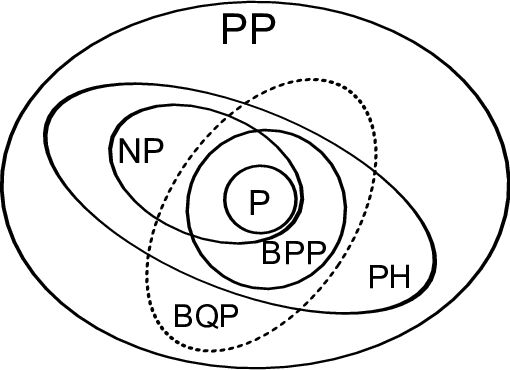
\includegraphics[scale=0.35]{bqp-inclusions.png}
        \caption{Inclusions connues et supposées de BQP}
    \end{figure}
\end{frame}

\subsection{Rapport à la thèse de Church-Turing}
\begin{frame}{Rapport à la thèse de Church-Turing}
    \begin{thesis}[Thèse de Church-Turing]
        Une fonction sur les entiers naturels peut être calculée si et seulement si elle est calculable par une machine de Turing.
    \end{thesis}
    \begin{thesis}[Thèse étendue de Church-Turing]
        Une machine de Turing probabiliste peut efficacement simuler tout modèle de calcul réaliste.
    \end{thesis}
    \begin{thesis}[Thèse quantiquement-étendue de Church-Turing]
        Tout système de calcul physique peut être efficacement simulé par une machine de Turing quantique.
    \end{thesis}
\end{frame}

\section{Algorithme de Deutsch-Jozsa}
\begin{frame}{Description du problème}
    On considère une fonction $f$ fonctionnant sur $n$ bits ou qubits:
    \begin{equation*}
        f : \{ 0, 1 \}^n \to \{ 0, 1 \}
    \end{equation*}
    Cette fonction est supposée être soit \emph{constante}, soit \emph{équilibrée}:
    \begin{equation*}
        |f^{-1}(\{0\})| = n \lor |f^{-1}(\{1\})| = n \lor \left(|f^{-1}(\{0\})| = |f^{-1}(\{1\})| = \frac{n}{2}\right)
    \end{equation*}
    (C'est à dire qu'elle produit soit que des \texttt{0}, soit que des \texttt{1}, soit exactement la moitié de \texttt{0} et l'autre moitié de \texttt{1}.)
\end{frame}

\begin{frame}{Solution classique}
    Dans le pire cas, un algorithme classique déterministe doit mesurer plus de la moitié des valeurs de $f$ pour les $2^n$ valeurs entrées possibles, i.e. $2^{n-1}+1$; la meilleure complexité en temps est dès lors exponentielle. (Néanmoins, ce problème peut être résolu avec une probabilité élevée avec un algorithme probabiliste, le problème est donc dans $BPP$.)
\end{frame}

\begin{frame}{Algorithme de Deutsch}
    On suppose que $f$ est implémentée par une porte sous la forme:
    \begin{equation*}
        f : \ket{x}\ket{y} \mapsto \ket{x}\ket{f(x)\oplus y}
    \end{equation*}
    \begin{figure}[!ht]
        \centering
        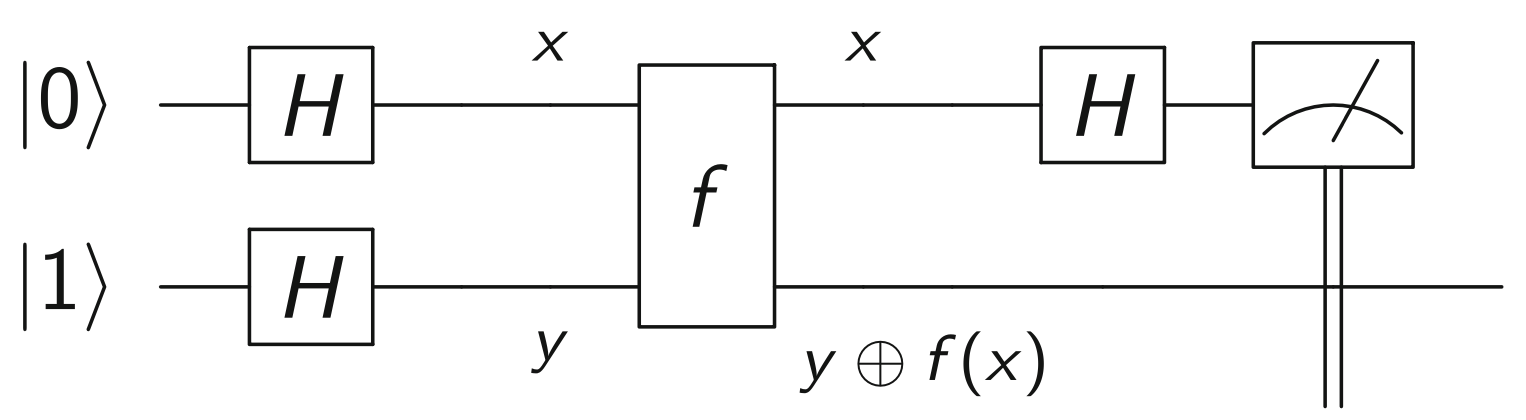
\includegraphics[scale=0.4]{deutsch-circuit.png}
        \caption{Circuit de l'algorithme de Deutsch}
    \end{figure}
\end{frame}

\begin{frame}{Algorithme de Deutsch}
    L'état du premier qubit est finalement:
    \begin{equation*}
        \frac{1}{2} \big[ \big(1+(-1)^{f(0)\oplus f(1)}\big)\ket{0} + \big(1-(-1)^{f(0)\oplus f(1)}\big)\ket{1} \big]
    \end{equation*}
    qui vaut $\ket{0}$ si et seulement $f(0)\oplus f(1) = 0$.
\end{frame}

\begin{frame}
    \frametitle{Cas général ($n$ quelconque)}
    \begin{figure}[!ht]
        \centering
        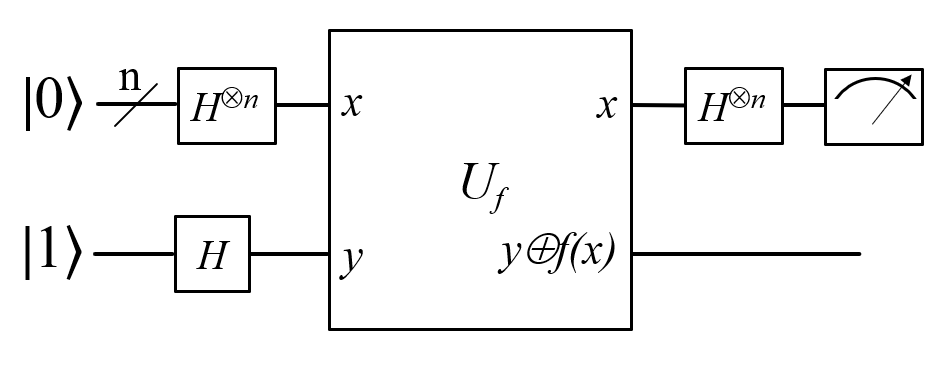
\includegraphics[scale=0.5]{deutsch-circuit-n.png}
        \caption{Circuit de l'algorithme de Deutsch}
    \end{figure}
\end{frame}

\end{document}